\documentclass[a4paper, notitlepage, 12pt]{scrartcl}
\author{Lukas Rost \\ \small{Teilnahme-ID: 44137}}
\title{Aufgabe 2 \\ \glqq Wehret den Wildschweinen!\grqq  - Dokumentation}
\subtitle{36. Bundeswettbewerb Informatik 2017/18 - 2. Runde \\~\\}
\date{9. April 2018}
\usepackage[ngerman]{babel}
\usepackage[utf8]{inputenc}
\usepackage{graphicx}
\usepackage{wrapfig}
\usepackage{color}
\usepackage[dvipsnames]{xcolor}
\usepackage{hyperref}
\usepackage[top=2.5cm, bottom=2cm, left=2.5cm, right=2.5cm]{geometry}
\usepackage{fancyvrb}
\usepackage{caption}
\usepackage{mathtools}
\usepackage{fancyhdr}
\usepackage{lastpage}
\usepackage{amsthm}
\usepackage{multicol}
\usepackage{longtable}
\usepackage{tabu}
\usepackage{minted}
\fvset{breaklines=true}

\pagestyle{fancy}
\lhead{Lukas Rost, Teilnahme-ID: 44137}
\rhead{Aufgabe 2, Seite \thepage ~von \pageref{LastPage}}
\cfoot{ }

\newenvironment{longlisting}{\captionsetup{type=listing}}{}

\newmintedfile{python}{frame=single,linenos,samepage=false,firstnumber=1,rulecolor=\color{Gray},autogobble,breakafter=.\]),fontsize=\footnotesize}

\begin{document}
\renewcommand{\contentsname}{\centerline{Inhaltsverzeichnis}}
 \maketitle
 \tableofcontents
 \thispagestyle{empty}
 \newpage
 \setcounter{page}{1}
 
 \section{Lösungsidee}
 \subsection{Umformung des Problems in ein Min-Cut-Problem}
 \label{sec:umform}
 Die Matrix der Planquadrate lässt sich als gerichteter und kantengewichteter Graph $G = \{V,E\}$ darstellen, für den gilt:
 \begin{itemize}
 \item Die Menge der Knoten $V$ entspricht der Menge aller Planquadrate in der Matrix.
 \item Die Menge der Kanten $E$ enthält für jeden Knoten eine gerichtete Kante zu seinen oben, unten, links und rechts benachbarten Knoten, sofern diese existieren. Das Gewicht einer solchen Kante wird definiert als $ 1 - \Delta h$, \footnote{Hier ließe sich anstatt 1 Meter auch jeder beliebige andere Höhenunterschied einsetzen, der dann von den Wildschweinen nicht überwindbar ist.} wobei $\Delta h$ den Betrag des Höhenunterschieds zwischen den verbundenen Knoten darstellt. Somit entspricht das Gewicht der Kante dem Höhenunterschied, der zwischen den beiden Knoten noch hinzugewonnen werden müsste, um den Übergang zwischen ihnen unpassierbar zu machen. Hätte eine Kante ein Gewicht $\leq 0$, so wird diese nicht zum Graphen hinzugefügt, da der Übergang zwischen diesen Knoten schon im Ursprungszustand unpassierbar ist.
 \item Es werden zwei zusätzliche Knoten $s$ (Quelle) und $t$ (Senke) definiert. Die Quelle stellt dabei bildlich gesprochen den Wald dar, aus dem die Wildschweine kommen und die Senke repräsentiert den Acker, den die Wildschweine erreichen wollen.
 \item Es werden gerichtete Kanten zum Graphen hinzugefügt, die von $s$ zu jedem Knoten in der ersten Reihe\footnote{Reihen verlaufen von links/Westen nach rechts/Osten, Spalten von oben/Norden nach unten/Süden.} der Matrix verlaufen, da die Wildschweine ja immer über diese Reihe das Brachland betreten. Weiterhin werden ebensolche Kanten von jedem Knoten in der letzten Reihe zu $t$ hinzugefügt, da die Wildschweine über diese Reihe das Brachland verlassen. Allen diesen Kanten wird als Gewicht $\infty$ zugewiesen.\footnote{Diese Vorgehensweise entspricht derjenigen für das Max-Flow- bzw. Min-Cut-Problem mit mehreren Quellen und Senken, da eigentlich die gesamte erste Reihe die Quellen und die gesamte letzte Reihe die Senken darstellt.\cite{Src:Multiple}}
 \end{itemize}
Nun stellt der Graph ein Flussnetzwerk dar, welches im nächsten Abschnitt genauer erklärt wird. In diesem Netzwerk entspricht das Problem der kostengünstigsten Erdarbeiten dem Problem des minimalen s-t-Schnitts. Ein s-t-Schnitt ist dabei definiert als eine Aufteilung der Knoten senkrecht zum Netzwerkfluss in zwei disjunkte Teilmengen $S$ und $T$, für die gilt $s\in S$ und $t\in T$. Ein minimaler Schnitt ist ein solcher Schnitt, sodass die Summe der Kantenkapazitäten bzw. Kantengewichte von $S$ nach $T$ minimal wird. Es gilt also, dass \begin{equation}c(S,T) = \sum_{u \in S, v \in T \wedge (u,v) \in E} c(u,v)\end{equation} für keinen anderen Schnitt kleiner ist. \cite{Src:tre} Die Kanten dieses Schnitts geben dann an, zwischen welchen Feldern Erde verschoben werden muss, um so kostengünstig wie möglich das Brachland unpassierbar zu machen. \\ \\ 
Dadurch, dass die Kanten zu s und zu t ein Gewicht von $\infty$ haben, werden diese keinesfalls Teil des minimalen Schnitts sein. Ebensowenig werden Kanten, die innerhalb der ersten oder letzten Reihe verlaufen, dem minimalen Schnitt angehören, da dann auch Kanten zu s bzw. t Teil dieses Schnitts wären, was (s.o.) ausgeschlossen ist. Somit gibt der Schnitt in jedem Fall Erdarbeiten an, die, egal von welchem Planquadrat der ersten bzw. letzten Reihe das Brachland betreten bzw. verlassen wird, das Brachland unpassierbar machen. Ein Beispiel eines so gebildeten Netzwerkes mit $n=3$ ist in der folgenden Abbildung zu sehen.
\begin{figure}[H]
\centering 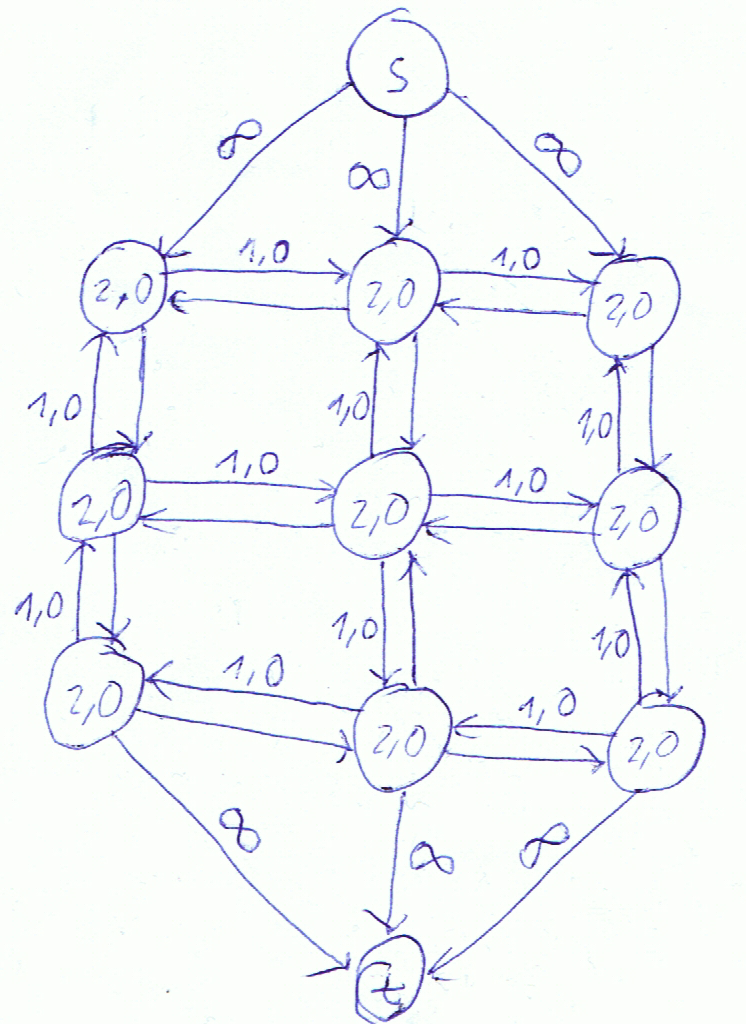
\includegraphics[width=0.4\textwidth]{pics/ill-graph.png}
\end{figure}
 \subsection{Grundlegende Informationen zu Flussnetzwerken}
Ein Flussnetzwerk ist ein gerichteter Graph $G = \{V,E\}$ mit einer charakteristischen Quelle $s$ und einer Senke $t$ sowie einer Kapazitätsfunktion $e \rightarrow c(e)$, die jeder Kante eine nichtnegative reelle Zahl zuweist. In unserem Fall entspricht die Kapazität einer Kante dem Gewicht dieser.
Über dieses Netzwerk kann ein Fluss gelegt werden. Dieser muss folgende Bedingungen erfüllen:
\begin{itemize}
 \item Ein Fluss hat eine Flusswertfunktion $e \rightarrow f(e)$, die jeder Kante einen nicht negativen Wert $f(e)$ zuweist. Der Flusswert $f(e)$ ist maximal so groß wie seine Kapazität, d. h. für für jede Kante $e \in E$ gilt $f(e) \leq c(e)$.
\item Für jeden Knoten (außer der Quelle $s$ und der Senke $t$) gilt der Flusserhalt: Für alle Kanten, die in einen Knoten gehen, ist die Summe der Werte f(e) genauso groß wie bei den Kanten, die aus einem Knoten gehen. Mathematisch lässt sich dies wie folgt formulieren ($e \in E$ und ($v \in V$)):
\begin{equation} \forall v,e \in G\backslash\{s,t\} : \sum_{\text{e führt nach v}} f(e) = \sum_{\text{e führt weg von v}} f(e) \end{equation}
\item Der Abfluss von der Quelle S ist gleich dem Zufluss zu der Senke t. Es gilt somit ($e \in E$):
\begin{equation} \forall e \in G : \sum_{\text{e führt weg von s}} f(e) = \sum_{\text{e führt nach t}} f(e) \end{equation}
Der Abfluss von $s$ bzw. der Zufluss zu $t$ wird als Wert des Flusses $|f|$ bezeichnet.
\item  Ein Fluss ist genau dann maximal, wenn bei keinem anderen Fluss in dem Graphen $|f|$ größer ist.
\end{itemize}
Mithilfe des maximalen Flusses lässt sich nun ein minimaler s-t-Schnitt in diesem Graphen bestimmen. Nach dem Max-Flow-Min-Cut-Theorem gilt zwischen diesen der Zusammenhang, dass ein maximaler Fluss genau den Wert eines minimalen Schnitts hat. Dies lässt sich folgendermaßen beweisen:
\begin{proof}[Beweisskizze]
Der Fluss, der über einen Schnitt fließt, hat den Wert des gesamten Flusses, da ein Schnitt den Graphen in zwei Teilmengen teilt und somit der gesamte Fluss zwischen $s$ und $t$ über diesen Schnitt geflossen sein muss. Daraus folgt, dass der Flusswert maximal so groß sein kann wie die Kapazität dieses Schnittes. \\
Nun betrachtet man den Fluss $f$. Wenn dieser nicht maximal wäre, gäbe es noch irgendeine Möglichkeit, den Fluss über irgendeinen Pfad zu erhöhen. Wäre $f$ nun maximal, kann diese Eigenschaft folglich nicht mehr auftreten, d. h. über einen Schnitt ist die Kapazität des Schnittes gleich dem darüber
fließenden Fluss. \\ Da der Fluss über dem Schnitt stets gleich ist, folgt daraus, dass es sich hierbei um den
minimalen Schnitt handelt. Dadurch ist die Behauptung belegt.
\end{proof}
Zum Verständnis des im nächsten Abschnitt behandelten Algorithmus müssen noch die Begriffe \textit{Residualnetzwerk} und \textit{augmentierender Pfad} definiert werden.
\\ \\
\textbf{Residualnetzwerk:} Es sei $G$ der ursprüngliche Graph und $f$ ein Fluss auf diesem. Des weiteren sei $e$ eine Kante von $v$ zu $w$  in $G$ mit der Kapazität $c(e)$. Dann ist das Residualnetzwerk wie folgt definiert:
\begin{itemize}
\item Zunächst wird der ursprüngliche Graph mit allen Knoten und Kanten kopiert.
\item Für jede Kante, auf der der Fluss $> 0$ ist, wird eine Rückkante (von $w$ nach $v$) in das Residualnetzwerk eingefügt. Man setze die Kapazität dieser Rückkante auf $f(e)$. Sofern die Rückkante schon existiert, addiere man $f(e)$ zur bisherigen Kapazität.
\item Wenn $f(e) < c(e)$, setze man für die Kante $e$ die Kapazität $c(e) - f(e)$
\end{itemize}
Somit gibt im Residualnetzwerk die Kapazität einer Hinkante an, um wie viel der Fluss auf ihr noch erhöht werden darf, während die Kapazität einer Rückkante angibt, um wie viel der Fluss auf der zugehörigen Hinkante verringert werden darf. Im im letzten Abschnitt beschriebenen, hier benutzten Netzwerk existiert offensichtlich zu jeder Kante schon eine Rückkante, die gemäß der obigen Definition auch im Residualnetzwerk als solche dient.
\\ \\
\textbf{augmentierender Pfad:} Unter Augmentieren versteht man grundsätzlich das Erhöhen des Flusses über eine Kante. Ein augmentierender Pfad ist somit ein Pfad zwischen $s$ und $t$, über den der Fluss erhöht werden kann. Das Residualnetzwerk hilft dabei, noch nicht ausgelastete augmentierende Pfade zu finden.
 \subsection{Mögliche Umsetzung durch den Edmonds-Karp-Algorithmus}
Grundsätzlich muss zur Bestimmung eines minimalen Schnitts zuerst der maximale Fluss berechnet werden. Aus dem dabei entstandenen Residualnetzwerk lässt sich schließlich der minimale Schnitt ableiten.
\\ \\
Zur Berechnung des maximalen Flusses habe ich den Edmonds-Karp-Algorithmus gewählt. Dieser ist einfach und leicht verständlich und obwohl alternative Algorithmen mit einer teilweise schnelleren Laufzeit existieren, ist der Edmonds-Karp-Algorithmus für die Bearbeitung dieser Aufgabe völlig ausreichend. Eine Übersicht über alternative Algorithmen findet man unter \cite{Src:gft}. Die Laufzeit des Edmonds-Karp-Algoritmus wird in Teilkapitel 1.5 bestimmt.
\\ \\
Grundlegend entspricht der Edmonds-Karp-Algoritmus dem Algorithmus von Ford und Fulkerson, weshalb dieser zuerst besprochen wird. Er arbeitet wie folgt:
\begin{enumerate}
\item Initialisiere mit dem Nullfluss, d.h. setze für jede Kante $e \in E$  $f(e)=0$.
\item Solange es im Residualnetzwerk $G_{f}$ einen Pfad von $s$ nach $t$ gibt, bestimme einen solchen Pfad $P$ und tue:
\begin{enumerate}
\item Bestimme $\gamma$ als Minimum der Residualkapazitäten auf $P$.
\item Augmentiere diesen Pfad soweit wie möglich, d.h. setze für alle Kanten auf $P$  $f(e) = f(e) + \gamma$ und für alle Rückkanten zu diesen setze $f(e) = f(e) - \gamma$.
\end{enumerate}
\end{enumerate}
Der Ford-Fulkerson-Algorithmus lässt offen, wie ein solcher augmentierender Pfad bestimmt wird. Der Edmonds-Karp-Algorithmus legt fest, dass stets der kürzeste Pfad (nach der Anzahl der enthaltenen Kanten) genutzt wird. In den meisten Implementierungen geschieht dies über eine Breitensuche oder eine Abwandlung dieser. So wird auch in meiner Implementierung eine bidirektionale Breitensuche genutzt, die gleichzeitig von $s$ und von $t$ aus sucht und genau dann einen Pfad gefunden hat, wenn beide Teile sich an einem Knoten treffen. Damit lässt sich die Laufzeit der Suche weiter reduzieren.
\\ \\
Sobald der Edmonds-Karp-Algorithmus terminiert, kann aus dem Residualgraphen einfach der minimale Schnitt bestimmt werden. Alle Kanten, die im Residualgraphen eine Kapazität von 0 haben, beschreiben den minimalen Schnitt. Auf diesen entspricht im ursprünglichen Graphen der Fluss der Kapazität, sie sind also \glqq gesättigt\grqq . Da durch den minimalen Schnitt (s. o.) der gesamte Fluss fließen muss und, da es sich um einen minimalen Schnitt handelt, diese Kanten auch maximal ausgelastet sein müssen, entspricht der minimale Schnitt genau den im ursprünglichen Graphen gesättigten Kanten.
\\ \\
Wenn man nun diese Kanten aus dem Graphen entfernt, bilden diejenigen Knoten, die von $s$ erreichbar sind, die erste Teilmenge. Alle restlichen Knoten bilden die zweite Teilmenge. Die Erreichbarkeit lässt sich einfach per Breitensuche bestimmen.
 \subsection{Nutzung des minimalen Schnitts zur Lösung des Problems}
 \label{sec:loesprob}
Hat man nun den minimalen Schnitt des Graphen bestimmt, kann man aus diesem die notwendigen Erdarbeiten ableiten. Hier gibt es zunächst einmal den Fall, dass der minimale Schnitt einen Wert von 0 hat. Dann hat der maximale Fluss denselben Wert, was bedeutet, dass kein Fluss zwischen Oberseite ($s$) und Unterseite ($t$) möglich ist. Also ist die Matrix schon unpassierbar und muss nicht mehr verändert werden. \\ \\
Ist dies nicht der Fall, so sind offensichtlich noch Erdarbeiten nötig. Um zu bestimmen, wo diese stattfinden müssen, benötigt man die Kanten des minimalen Schnitts, also alle Kanten, die von der einen in die andere Teilmenge verlaufen. \\ \\
Entlang jeder dieser Kanten muss Erde verschoben werden. Dabei wird vom Planquadrat mit der geringeren Höhe zum höheren Planquadrat genau die Hälfte der oben bestimmten Kantenkapazität $ 1 - \Delta h$ an Erde verschoben. \footnote{Diese muss hier neu bestimmt werden, da sich diese aufgrund vorheriger Veränderungen an der Matrix geändert haben könnte.} Dadurch erhöht sich die Höhe des höheren Planquadrats um $ \frac{1 - \Delta h}{2}$ und die Höhe des niedrigeren Planquadrats sinkt um ebensoviel. Dadurch erhöht sich $\Delta h$ auf $1$, und dieser Übergang ist nicht mehr passierbar. \\ \\
Diese Vorgehensweise führt jedoch in einem Sonderfall nicht zum Erfolg. Wenn der minimale Schnitt wie im folgenden Bild dargestellt, also quasi treppenförmig, verläuft, kann dies unter Umständen dazu führen, dass das Brachland immer noch passierbar bleibt. Dies ist genau dann möglich, wenn in dieser Konstellation in der originalen Matrix drei Planquadrate existieren, sodass sich das höchste und das niedrigste Quadrat auf einer Seite des Schnitts befinden, aber das Quadrat mit mittlerer Höhe auf der anderen Seite liegt. Zusätzlich müssen Kanten, also Übergangsmöglichkeiten vom niedrigsten zum mittleren und vom mittleren zum höchsten Quadrat bestehen.
\begin{figure}[H]
\centering 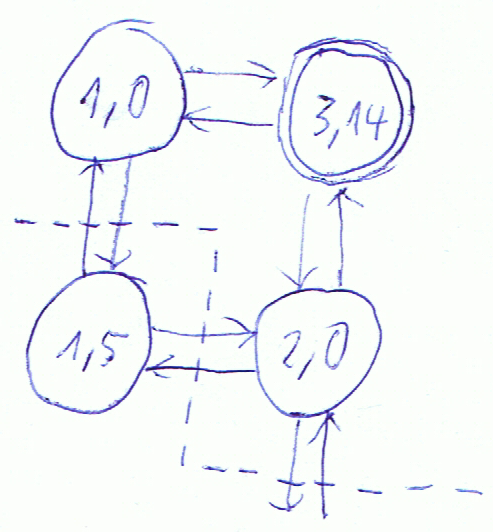
\includegraphics[width=0.3\textwidth]{pics/ill-cut.png}
\end{figure}
Dann nämlich wird der oben dargestellte Schritt beispielsweise zwischen dem mittleren und den niedrigsten Quadrat ausgeführt, jedoch erfolgt der gleiche Schritt auch zwischen dem mittleren und dem höchsten Quadrat, was den vorherigen Schritt wieder aufhebt und eine neue Passiermöglichkeit schafft. Im Beispiel verändert sich die Höhe des niedrigsten Quadrats von 1,0 auf 0,75 und die des mittleren Quadrats von 1,5 auf 1,75. Anschließend wird dann jedoch die Höhe des mittleren Quadrats auf 1,375 geändert (und $1,375 - 0,75 < 1,0 $ !) und die des höchsten Quadrats auf 2,375. Um dies zu vermeiden, führt man den ersten Schritt normal aus, erreicht jedoch die benötigte Höhenänderung im zweiten Schritt dadurch, dass man Erde von einem anderem Nachbarquadrat des höchsten Quadrats verschiebt. \footnote{Genaugenommen ist in einem solchen Fall der Algorithmus nicht 100-prozentig sicher optimal, da dies nicht in unserem Graph modelliert werden kann. Somit könnte es theoretisch noch eine optimalere Möglichkeit zum Verschieben der Erde geben. In diesem Fall ist der Algorithmus jedoch zumindest eine gute Heuristik.} Dieses Nachbarquadrat sollte sinnvollerweise nicht dem Endknoten einer Kante des Schnitts entsprechen. Im obigen Beispiel könnte dies der doppelt umrandete Knoten sein.
 \subsection{Laufzeitanalyse des Algorithmus}
Es ist leicht zu erkennen, dass der Edmonds-Karp-Algorithmus den größten Anteil zur Laufzeit beiträgt. Alle anderen Operationen sind nicht der Rede wert. Zunächst ist leicht zu erkennen, dass die Anzahl der Knoten im Graphen $|V| = n^{2}$ ist (abhängig von der Seitenlänge der Matrix $n$), da die Matrix quadratisch ist und somit $n^{2}$ Planquadrate enthält. Zusätzlich kommen noch $s$ und $t$ dazu, welche jedoch im folgenden vernachlässigbar sind. \\ \\
Weiterhin befinden sich höchstens $|E| = 2 \cdot n + 2 \cdot n \cdot (n-1) = 2 \cdot n + 2 \cdot n^{2} - 2 \cdot n = 2 \cdot n^{2} $ Kanten im Graphen. Im Einzelnen sind dies die jeweils $n$ Kanten, die $s$ als Ausgangspunkt bzw. die $t$ als Endpunkt haben. Weiterhin befinden sich in der Matrix maximal $n \cdot (n-1)$ Kanten von links nach rechts und ebensoviele von oben nach unten. Die doppelt vorhandenen Kanten (in beide Richtungen) werden im Algorithmus als eine Kante und demzufolge hier auch so gezählt. \\ \\
Der Edmonds-Karp-Algorithmus hat nach Literaturangaben eine Laufzeit in $\mathcal{O}(|V| \cdot |E|^{2})$. Setzt man nun die Werte für $|V|$ und $|E|$ ein, so ergibt sich eine Laufzeit von $\mathcal{O}(4 \cdot n^2 \cdot n^4)$. Da konstante Faktoren vernachlässigbar sind, erhält man eine Laufzeit in $\mathcal{O}(n^6)$. Diese Laufzeit ist für die hier zu lösenden Beispiele mit Seitenlängen bis 20 absolut ausreichend und kann selbst größere Graphen in einer annehmbaren Laufzeit lösen. Hier ließe sich natürlich durch Max-Flow-Algorithmen mit geringerer Laufzeit noch eine Verbesserung erreichen. \\ \\
Die genannte Laufzeit von $\mathcal{O}(|V| \cdot |E|^{2})$ lässt sich folgendermaßen nachweisen: 
\begin{proof}[Nachweis]
Zunächst kann man zeigen, dass die Anzahl der zu augmentierenden Pfade des Edmonds-Karp-Algorithmus höchstens $\frac{|V| \cdot |E|}{2}$ beträgt. Dabei gibt es beim Augmentieren eines Pfades mindestens immer eine Kante, die gänzlich aus dem Residualnetzwerk gelöscht wird, da entweder eine Vorwärtskante vorkommt, die vollkommen gefüllt wird oder auch eine Rückwärtskante, die im Gegenzug geleert wird. Solch eine Kante bezeichne man als kritische Kante. Jedes Mal, wenn solch eine Kante eine kritische Kante ist, muss sich die Länge des durch diese Kante augmentierenden Pfades um 2 erhöhen. Da solch ein augmentierender Pfad höchstens die Länge n hat, können auf jeder Kante maximal $\frac{|V|}{2}$ augmentierende Pfade liegen, sodass die Gesamtzahl der augmentierenden Pfade höchstens $\frac{|V| \cdot |E|}{2}$ beträgt. Da die Breitensuche höchstens $|E|$ Kanten untersucht, folgt, dass der Algorithmus eine Laufzeit von $\mathcal{O}(|V| \cdot |E|^{2})$ hat.
\end{proof}
Zusätzlich soll hier auch die Speicherkomplexität betrachtet werden. Die Matrix selbst nimmt $\mathcal{O}(n^{2})$ Speicherplatz ein. Der Graph an sich nimmt bei Speicherung in einer Adjazenzliste $\mathcal{O}(|V| + |E|) = \mathcal{O}(n^{2})$ (Berechnung $|V|$ und $|E|$ siehe oben) Speicherplatz ein. Insgesamt ergibt sich, da Matrix und Graph die speicheraufwendigsten Datenstrukturen sind, eine quadratische Speicherkomplexität.
\subsection{Erweiterung}
Nehmen wir einmal an, die Wildschweine hätten eine Art von Intelligenz entwickelt und könnten einen Computer bedienen. Dieses Wissen wollen sie nun nutzen, um das Brachland zu passieren und dabei einen möglichst geringen Gesamthöhenunterschied zu überwinden. Weiterhin könnte für sie eventuell der größte Einzelhöhenunterschied auf diesem Weg von Interesse sein, denn dann könnten sie entsprechend dafür trainieren, das Brachland passieren zu können. Sie könnten dabei eventuell am Zustand vor den Erdarbeiten ebenso wie am Zustand nach den Erdarbeiten interessiert sein.\footnote{Ja, ich gebe zu, dieses Einsatzszenario ist etwas unrealistisch. ;-)}\\ \\
Zur Lösung dieses Problems kann man die oben dargestellte Formulierung als Graph im Prinzip weiterverwenden. Es müssen dabei jedoch folgende Änderungen vorgenommen werden:
\begin{itemize}
\item Kanten zu benachbarten Knoten erhalten nun das Gewicht $\Delta h$, wobei $\Delta h$ weiterhin der Betrag des Höhenunterschieds ist. Auch werden solche Kanten immer hinzugefügt, unabhängig von ihrem Gewicht.
\item Kanten, welche vorher das Gewicht $\infty$ hatten, erhalten nun das Gewicht $0$.
\end{itemize}
Nun entspricht das Problem dieser Erweiterung dem Problem des kürzesten Pfades zwischen zwei Knoten in einem Graphen (in diesem Fall $s$ und $t$). Dieses Problem kann beispielsweise durch den Dijkstra-Algorithmus gelöst werden. Dieser arbeitet grundlegend wie folgt:
\begin{enumerate}
\item Weise allen Knoten die beiden Eigenschaften „Distanz“ und „Vorgänger“ zu. Initialisiere die Distanz im Startknoten $s$ mit 0 und in allen anderen Knoten mit $\infty$.
\item Solange es noch unbesuchte Knoten gibt, wähle darunter denjenigen mit minimaler Distanz aus und
\begin{enumerate}
\item speichere, dass dieser Knoten schon besucht wurde.
\item Berechne für alle noch unbesuchten Nachbarknoten die Summe des jeweiligen Kantengewichtes und der Distanz im aktuellen Knoten.
\item Ist dieser Wert für einen Knoten kleiner als die dort gespeicherte Distanz, aktualisiere sie und setze den aktuellen Knoten als Vorgänger.
\end{enumerate}
\end{enumerate}
Wenn hierbei der gesuchte Knoten $t$ im Schritt 2 der aktive ist, kann dann schon abgebrochen werden.
Der Dijkstra-Algorithmus hat eine Laufzeit von $\mathcal{O}((|V|+|E|) \cdot \log |V|)$ (bei Implementierung mit einer Vorrangwarteschlange), was gemäß den obigen Berechnungen $\mathcal{O}(n^{2} \cdot \log n)$ entspricht. \\ \\ Da der Algorithmus den entsprechenden Weg durch das Setzen eines Vorgängers ebenfalls bestimmt, kann auch dieser selbst ausgegeben werden. Das Bestimmen der Einzelkante mit dem größten Gewicht auf diesem Pfad erfolgt dann durch Iterieren über alle Kanten des Pfades und die Suche des Maximums von deren Gewichten. \\ \\
Eine weitere mögliche Erweiterung wäre es, die Zäune an der linken und rechten Seite des Brachlands zu \glqq öffnen\grqq ~und zuzulassen, dass Wildschweine auch von links kommen sowie das Brachland nach rechts verlassen können. Dazu müsste man $s$ mit allen Knoten in der ersten Spalte und alle Knoten in der letzten Spalte mit $t$ verbinden. Die Kantengewichte werden wie beschrieben verteilt, anschließend könnte man den Edmonds-Karp-Algorithmus normal ausführen. Diese Erweiterung wurde nicht implementiert.
\begin{thebibliography}{xx}
\bibitem[1] {Src:CPH} Antti Laaksonen: Competitive Programmer’s Handbook, Kapitel 20 behandelt Flüsse, \url{https://cses.fi/book.html} 
\bibitem[2] {Src:ADM} Steven S. Skiena: The Algorithm Design Manual, ISBN 978-1-84800-069-8, Kapitel 6.5 und 15.8 bzw. 15.9 beschäftigen sich mit Fluss- und Schnittproblemen
\bibitem[3] {Src:sf} Steven Halim und Felix Halim: Competitive Programming, Kapitel 4.8 beschäftigt sich mit dem Edmonds-Karp-Algorithmus, \url{http://www.comp.nus.edu.sg/~stevenha/myteaching/competitive_programming/cp1.pdf}
\bibitem[4] {Src:gjt} Thomas Ottmann und Peter Widmayer: Algorithmen und Datenstrukturen, ISBN 978-3-662-55649-8, Kapitel 9.7 beschäftigt sich mit Flüssen
\bibitem[5] {Src:htt} Wikipedia-Artikel zum Ford und Fulkerson-Algorithmus, \url{https://de.wikipedia.org/wiki/Algorithmus_von_Ford_und_Fulkerson}
\bibitem[6] {Src:gft} Wikipedia-Artikel zur allgemeinen Übersicht über Flüsse in Netzwerken, \url{https://de.wikipedia.org/wiki/Fl\%C3\%BCsse_und_Schnitte_in_Netzwerken}
\bibitem[7] {src:hgf} Wikipedia-Artikel zum Maximum Flow Problem, \url{https://en.wikipedia.org/wiki/Maximum_flow_problem}
\bibitem[8] {Src:tre} Wikipedia-Artikel zum Max-Flow-Min-Cut-Theorem, \url{https://de.wikipedia.org/wiki/Max-Flow-Min-Cut-Theorem}
\bibitem[9] {Src:Multiple} Dokument zum Max-Flow-Problem für mehrere Quellen und Senken, \url{http://www.ifp.illinois.edu/~angelia/ge330fall09_maxflowl20.pdf}
\bibitem[10] {Src:dijk} Wikipedia-Artikel zum Dijkstra-Algorithmus, \url{https://de.wikipedia.org/wiki/Dijkstra-Algorithmus}
\end{thebibliography}
 \section{Umsetzung}
 \subsection{Allgemeines zur Bedienung des Programms}
 Das Programm wurde in Python 3.6.3 implementiert. Zur Verwaltung des abstrakten Datentyps Graph benutze ich die Python-Bibliothek \texttt{NetworkX}, welche über \texttt{pip3 install networkx} installiert werden kann. Grundlegend benutzt diese Adjazenzlisten, abstrahiert den Zugriff auf den Graphen jedoch ein wenig, sodass sich viele Operationen leichter durchführen lassen. Alle weiteren verwendeten Bibliotheken sind üblicherweise vorinstalliert. Die Eingabe des Programms erfolgt über eine Abfrage des Eingabedateinamens auf der Konsole, die Ausgabe erfolgt dann automatisch in eine entsprechende Datei mit dem vorgegebenen Dateinamen. Als kleiner Zusatz ist es möglich, die unüberwindbare Steigung zu verändern (entsprechend \autoref{sec:umform}), was zu Beginn abgefragt wird.
 \subsection{Umsetzung des Edmonds-Karp-Algorithmus}
 Im Modul \texttt{boarflow.py} sind folgende relevanten Funktionen zur Berechnung des minimalen Schnitts enthalten.
 \begin{longtabu} to \linewidth {lX}
 Funktion & Beschreibung \\ \hline \hline \endhead
 breadth\_first\_search() & bestimmt mithilfe einer Breitensuche die von einem bestimmten Knoten aus erreichbaren Knoten. Dabei werden schon gesehene Knoten in einem Dictionary gespeichert, ebenso wie Knoten auf der aktuellen und der nächsten Ebene. Der Algorithmus besucht dann für jede Ebene alle noch nicht gesehenen Knoten und fügt deren Nachbarn als Besuchskandidaten für die nächste Ebene hinzu. Die Funktion wird dazu genutzt, die von der Quelle aus erreichbare Teilmenge der Knoten zu bestimmen.\\ \hline
 build\_residual\_network() & erstellt die Anfangsform des Residualnetzwerks. Dazu werden alle Knoten kopiert sowie alle Kanten mit den entsprechenden Kapazitäten ebenfalls. Zu allen Kanten werden dann Rückkanten mit einer Kapazität von 0 bzw. falls diese Rückkanten im ursprünglichen Graphen schon existieren, der entsprechenden Kapazität, eingefügt. Falls für eine Kante keine Kapazität angegeben ist, wird dafür $\infty$ angenommen. Für alle Kanten wird mit dem Nullfluss initialisiert. \\ \hline
 edmonds\_karp() & enthält den eigentlichen Edmonds-Karp-Algorithmus. Das hier genutzte Residualnetzwerk arbeitet dabei nicht mit Residualkapazitäten im klassischen Sinne, sondern kommt mit der Speicherung von normaler Kapazität und dem Fluss aus. In einer Schleife wird immer wieder eine bidirektionale Breitensuche nach einem augmentierenden Pfad gestartet. Solange diese Ergebnisse liefert, werden beide Teile des Pfades zu einem Pfad zusammengefügt. Dieser wird anschließend augmentiert.\\ \hline
 augment() & ist eine Unterfunktion von edmonds\_karp(). Sie wird dazu genutzt, einen Pfad zu augmentieren. Dazu wird zuerst das Minimum der Residualkapazitäten bestimmt, welche hierfür als $c(e) -f(e)$ bestimmt werden. Dann wird der Fluss auf den genutzten Hinkanten entsprechend erhöht und auf den Rückkanten dazu verringert. \\ \hline
 bidirectional\_bfs() & ist eine Unterfunktion von edmonds\_karp(). Diese bidirektionale Breitensuche sucht nach einem augmentierenden Pfad. Die Beschränkung auf augmentierende Pfade wird dabei dadurch erreicht, dass nur diejenigen Kanten benutzt werden  dürfen, auf denen der Fluss kleiner als die Kapazität ist. Der Grund für die Benutzung einer solchen Suche in diesem Programm ist, dass dadurch die Laufzeit des Algorithmus verbessert werden kann. Es muss dann im Prinzip nur zweimal die Hälfte des Graphen durchsucht werden, was schneller möglich ist, als einmal den ganzen Graphen zu durchsuchen.\\ \hline
 minimum\_cut() & In dieser Funktion wird der minimaler Schnitt des Graphen bestimmt. Dazu werden alle gesättigten Kanten entfernt ($f(e) = c(e)$) und dann per Breitensuche die Erreichbarkeit von der Quelle aus bestimmt. Diese Information wird genutzt, um den Graphen in zwei Teilmengen/Partitionen zu teilen. \\
 \end{longtabu}
 \subsection{Implementierung des Hauptprogramms}
Im Hauptprogramm \texttt{wildschweine.py} befinden sich bis auf einige Ausnahmen nahezu alle Anweisungen außerhalb von Funktionen, werden also einfach hintereinander ausgeführt. Zunächst wird die Eingabedatei eingelesen (dazu wird die Funktion \texttt{read()} benutzt) und die zurückgegebene Matrix wird kopiert, da sie im Programm verändert wird, jedoch später in ihrer ursprünglichen Fassung noch gebraucht wird. Nun wird die Zeitmessung gestartet. \\ \\
Daraufhin wird der Graph wie in \autoref{sec:umform} beschrieben erstellt. Dabei werden die Knoten im Format \glqq $x|y$\grqq ~benannt, um sie später wiederfinden zu können. Dabei ist $x$ die Reihe in der Matrix, beginnend bei 0 und $y$ die Spalte in der Matrix, ebenfalls beginnend bei 0. $s$ und $t$ sind entsprechend den Konventionen Quelle und Senke. Bei Kanten, deren Kapazität $\infty$ ist, wird diese, wie bereits beschrieben, nicht angegeben. Zu beachten ist hierbei auch, dass Kanten nur dann eingefügt werden dürfen, wenn sie auch wirklich passierbar wären (Kapazität $>$ 0). Dies wird aufgrund der Ungenauigkeit von Gleitkommazahlen durch Vergleich mit einem $\varepsilon$, hier $10^{-4}$ realisiert. \\
Anschließend wird der minimale Schnitt berechnet. Wenn dieser 0 ist, ist die Matrix schon unpassierbar und es kann abgebrochen werden. Sonst werden durch Iteration über alle Kanten diejenigen Kanten bestimmt, die von der ersten Teilmenge $S$ in die zweite Teilmenge $T$ führen. Diese sind die Kanten des minimalen Schnitts, die im folgenden benötigt werden. \\ \\
Nun wird gemäß der generellen Regel zum kostengünstigsten Verschieben (\autoref{sec:loesprob}) Erde verschoben. Dabei wird gleichzeitig gezählt, wie viel Erde verschoben wurde. Sollte zufällig über eine Kante weniger als keine Erde verschoben werden müssen, wurde diese Kante schon durch Erdarbeiten über eine andere Kante unpassierbar gemacht. Deshalb kann eine solche Kante ignoriert werden. Weiterhin werden zwei Listen geführt, die für jede Kante den jeweils höheren und den tieferen Knoten protokollieren. \\ \\
Nun muss noch der Sonderfall berücksichtigt werden. Dazu geht man alle Kanten durch und untersucht, ob der hier tiefere Knoten schon einmal ein höherer Knoten war. Dann entnimmt man der Liste der tieferen Knoten den zu diesem höheren Knoten gehörenden tieferen Knoten.\footnote{Klingt etwas unverständlich, funktioniert aber.} Diese drei Knoten (hier höherer Knoten, hier tieferer Knoten und der Knoten aus der Liste) entsprechen den in \autoref{sec:loesprob} genannten drei Planquadraten. Bei diesen stellt man nun die ursprüngliche Höhe wieder her und sortiert sie anschließend nach dieser. Dann wird entsprechend die Verschiebung zwischen tiefstem und mittlerem Planquadrat normal ausgeführt. Für die nötige Verschiebung zwischen mittlerem und höchstem Planquadrat wird mithilfe der Funktion \texttt{auswahl()} ein Nachbarfeld des höchsten Felds herangezogen, welches nicht am Schnitt und damit an Erdarbeiten beteiligt ist. \\ \\
Nun hat man eine unpassierbare Lösungsmatrix, welche ausgegeben wird. Außerdem wird die verschobene Erde (in cm), welchen den Kosten entspricht, sowie die benötigte Zeit ausgegeben.
\subsection{Implementierung der Erweiterung}
In der Datei zur Erweiterung \texttt{dijkstra.py} befindet sich die Funktion \texttt{shortest\_path()}. Diese erhält als Eingabe eine beliebige Matrix mit den Höhen. Anschließend wird gemäß den bereits genannten Regeln der Graph aufgebaut. Der Dijkstra-Algorithmus wird dann ausgeführt und gibt den kürzesten Weg und dessen Länge zurück. Nun wird durch Iterieren über alle Kanten des Weges diejenige mit minimalem Gewicht (entsprechend der minimalen Steigung) bestimmt. Anschließend werden minimale Steigung, Gesamtsteigung und der Weg selbst ausgegeben. Die Funktion wird für jede Eingabedatei sowohl für die Eingabematrix als auch für die Ausgabematrix aufgerufen. \\ \\
Der Dijkstra-Algorithmus selbst befindet sich in der Funktion \texttt{dijkstra\_st()}. Er arbeitet nach dem oben bereits beschriebenen Prinzip. Zur effizienten Implementierung wird hier eine Vorrangwarteschlange bzw. Priority Queue aus der Bibliothek \texttt{heapq} verwendet.
 \section{Beispiele}
 \RecustomVerbatimCommand{\VerbatimInput}{VerbatimInput}%
{fontsize=\footnotesize,
 %
 frame=lines,  % top and bottom rule only
 framesep=2em, % separation between frame and text
 rulecolor=\color{Gray},
 %
 label=\fbox{\color{Black} wildschwein1-lsg.txt},
 labelposition=topline,
 numbers=left,
 %
 commandchars=\|\(\), % escape character and argument delimiters for
                      % commands within the verbatim
 commentchar=*        % comment character
}
\VerbatimInput{../Bwinf-Aufgabe2-Wildschweine/wildschwein1-lsg.txt}
\RecustomVerbatimCommand{\VerbatimInput}{VerbatimInput}%
{fontsize=\footnotesize,
 %
 frame=lines,  % top and bottom rule only
 framesep=2em, % separation between frame and text
 rulecolor=\color{Gray},
 %
 label=\fbox{\color{Black} wildschwein2-lsg.txt},
 labelposition=topline,
 numbers=left,
 %
 commandchars=\|\(\), % escape character and argument delimiters for
                      % commands within the verbatim
 commentchar=*        % comment character
}
 \VerbatimInput{../Bwinf-Aufgabe2-Wildschweine/wildschwein2-lsg.txt}
 \RecustomVerbatimCommand{\VerbatimInput}{VerbatimInput}%
{fontsize=\footnotesize,
 %
 frame=lines,  % top and bottom rule only
 framesep=2em, % separation between frame and text
 rulecolor=\color{Gray},
 %
 label=\fbox{\color{Black} wildschwein3-lsg.txt},
 labelposition=topline,
 numbers=left,
 %
 commandchars=\|\(\), % escape character and argument delimiters for
                      % commands within the verbatim
 commentchar=*        % comment character
}
 \VerbatimInput{../Bwinf-Aufgabe2-Wildschweine/wildschwein3-lsg.txt}
  \RecustomVerbatimCommand{\VerbatimInput}{VerbatimInput}%
{fontsize=\footnotesize,
 %
 frame=lines,  % top and bottom rule only
 framesep=2em, % separation between frame and text
 rulecolor=\color{Gray},
 %
 label=\fbox{\color{Black} wildschwein4-lsg.txt},
 labelposition=topline,
 numbers=left,
 %
 commandchars=\|\(\), % escape character and argument delimiters for
                      % commands within the verbatim
 commentchar=*        % comment character
}
 \VerbatimInput{../Bwinf-Aufgabe2-Wildschweine/wildschwein4-lsg.txt}
   \RecustomVerbatimCommand{\VerbatimInput}{VerbatimInput}%
{fontsize=\footnotesize,
 %
 frame=lines,  % top and bottom rule only
 framesep=2em, % separation between frame and text
 rulecolor=\color{Gray},
 %
 label=\fbox{\color{Black} wildschwein5-lsg.txt},
 labelposition=topline,
 numbers=left,
 %
 commandchars=\|\(\), % escape character and argument delimiters for
                      % commands within the verbatim
 commentchar=*        % comment character
}
 \VerbatimInput{../Bwinf-Aufgabe2-Wildschweine/wildschwein5-lsg.txt}
 \begin{table}[H]
    \begin{tabular}{|c|c|c|} 
    \hline
    Beispiel                                      & benötigte Kosten & Laufzeit (ca.)       \\ \hline \hline
    wildschwein1.txt                              & 706.60 Euro      & 316 Millisekunden    \\
    wildschwein2.txt                              & 600.00 Euro      & 19 Millisekunden     \\
    wildschwein3.txt                              & 307.50 Euro      & 11 Millisekunden     \\
    wildschwein4.txt                              & 370.90 Euro      & 139 Millisekunden    \\
    wildschwein5.txt                              & 405.20 Euro      & 261 Millisekunden    \\
    eigenes Beispiel  (50 x 50)  test1\_50.txt    & 1031.00 Euro     & 11788 Millisekunden  \\
    eigenes Beispiel  (100 x 100)  test2\_100.txt & 4564.30 Euro     & 156630 Millisekunden \\ \hline
    \end{tabular}
\end{table}
Somit löst das Programm sämtliche vorgegebenen Beispiele in unter einer Sekunde. Diese Lösungen sind auch nachweisbar richtig, denn gibt man die Lösungsdateien wieder in das Programm ein, so wird anhand des minimalen Schnitts, welcher dann einen Wert von 0 hat, die Unpassierbarkeit der Lösungsmatrizen festgestellt. Die eigenen Beispiele sind der Implementierung zusammen mit deren Lösungsdateien beigelegt.
\\ \\
Weiterhin wurden mit dem beigelegten Skript \texttt{heatmap.py} Heatmaps für die Lösungen aller Beispiele erstellt, die einen Überblick über die Höhen der einzelnen Felder geben. Hierfür wurden \texttt{numpy} und \texttt{matplotlib} eingesetzt. Außerdem befinden sich im Ordner \texttt{extras} Bilder, die für jede Lösung zeigen, wo ungefähr die Barriere für die Wildschweine verläuft (s.u.). Teilweise scheint diese Barriere nicht ganz geschlossen zu sein, was jedoch damit zusammenhängt, dass dafür Daten über die Passierbarkeit von oben nach unten und von links nach rechts zusammengefügt wurden, welche nicht vollständig zueinander passen.
\\
Theoretisch ist es möglich, dass sich in den Ausgabedateien Werte durch Rundungsfehler im Millimeterbereich von den optimalen Werten unterscheiden. Diese Fehler sind jedoch völlig unerheblich.
\begin{multicols}{2}
\begin{figure}[H]
\centering 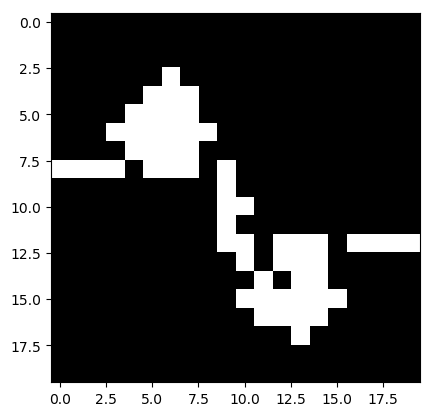
\includegraphics[width=0.5\textwidth]{pics/wildschwein1-lsg-top_to_bot_bool.png}
\end{figure}

\begin{figure}[H]
\centering 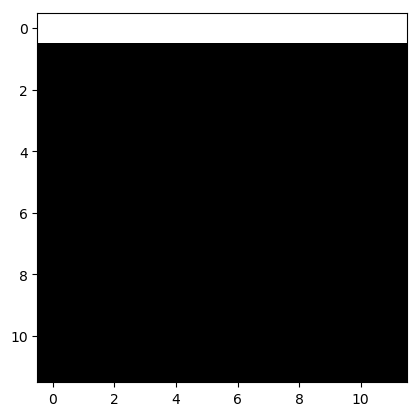
\includegraphics[width=0.5\textwidth]{pics/wildschwein2-lsg-top_to_bot_bool.png}
\end{figure}

\begin{figure}[H]
\centering 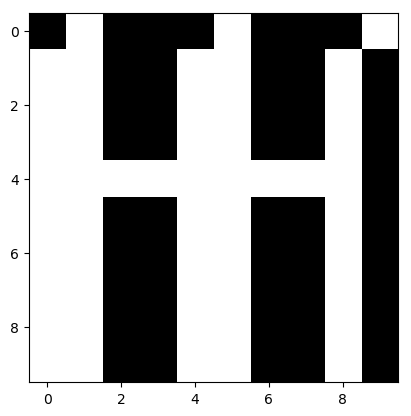
\includegraphics[width=0.5\textwidth]{pics/wildschwein3-lsg-top_to_bot_bool.png}
\end{figure}

\begin{figure}[H]
\centering 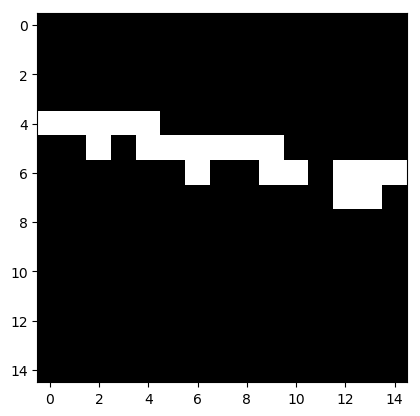
\includegraphics[width=0.49\textwidth]{pics/wildschwein4-lsg-top_to_bot_bool.png}
\end{figure}

\begin{figure}[H]
\centering 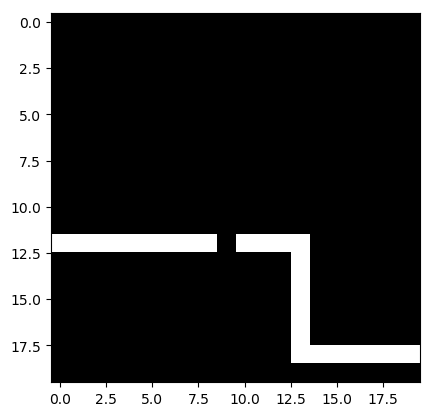
\includegraphics[width=0.5\textwidth]{pics/wildschwein5-lsg-top_to_bot_bool.png}
\end{figure}
~\\
\textit{Auf der vorigen Seite:} \\
Links: wildschwein1-lsg.txt \\
Rechts: wildschwein2-lsg.txt \\
\textit{Auf dieser Seite:} \\
Links oben: wildschwein3-lsg.txt \\
Links unten: wildschwein4-lsg.txt \\
Rechts oben: wildschwein5-lsg.txt \\
\end{multicols}
\newpage
\subsection{Ergebnisse der Erweiterung}
Der genaue Weg wurde ausgelassen, da er hier uninteressant ist.
\begin{table}[H]
    \begin{tabular}{|c|c|c|c|} 
    \hline
Beispiel & Gesamt-Höhenunterschied & größte Einzelsteigung \\ \hline
wildschwein1.txt & 0,59 & 0,058 \\
wildschwein1-lsg.txt & 2,35 & 1,0 \\
wildschwein2.txt & 0,0 & 0,0  \\
wildschwein2-lsg.txt & 1,5 & 1,0  \\
wildschwein3.txt & 0,0 & 0,0 \\
wildschwein3-lsg.txt & 1,178 & 1,11  \\
wildschwein4.txt & 2,508 & 0,554 \\
wildschwein4-lsg.txt & 3,381 & 1,0  \\
wildschwein5.txt & 5,71 & 0,646 \\
wildschwein5-lsg.txt & 5,883 & 1,0 \\
test1\_50.txt & 2,012 & 0,624 \\
test1\_50-lsg.txt & 2,482 & 1,0 \\
test2\_100.txt & 0,0 & 0,0 \\
test2\_100-lsg.txt & 2,0 & 1,0 \\ \hline
    \end{tabular}
\end{table}
 \section{Quellcode}
 \renewcommand{\listingscaption}{Quellcode}
 
 \begin{longlisting}
 \pythonfile[firstline=27,lastline=185]{../Bwinf-Aufgabe2-Wildschweine/wildschweine.py}
 \caption{Auszug aus dem Hauptprogramm (\textit{wildschweine.py}), soweit möglich ohne Eingabe und Ausgabe}
 \end{longlisting}
 
 \begin{longlisting}
 \pythonfile{../Bwinf-Aufgabe2-Wildschweine/boarflow.py}
 \caption{Das Modul zur Berechnung des minimalen Schnitts (\textit{boarflow.py})}
 \end{longlisting}
 
 \subsection{Quellcode der Erweiterung}
 \begin{longlisting}
 \pythonfile{../Bwinf-Aufgabe2-Wildschweine/dijkstra.py}
 \caption{Die Erweiterung (\textit{dijkstra.py})}
 \end{longlisting}
 \end{document}